\documentclass[12pt]{article}

\usepackage[T2A]{fontenc}
\usepackage[utf8]{inputenc}
\usepackage[russian]{babel}

\usepackage[a4paper,vmargin=18mm,lmargin=30mm,rmargin=10mm]{geometry}

\usepackage{graphicx}

\begin{document}

\begin{center}

Министерство науки и высшего образования Российской Федерации

\smallskip

ФГАОУ ВО <<УрФУ имени первого Президента России Б.Н. Ельцина>>

\medskip

\large

\textbf{РЕЦЕНЗИЯ}

на магистерскую диссертацию

Студента Корабельникова Алексея Алексеевича группы МЕНМ-280901
 
\medskip

\normalsize

\raggedright

\noindent
\textbf{Тема магистерской диссертации:} МНОГОМЕРНЫЙ АЛГОРИТМ ОВЫПУКЛЕНИЯ РОЯ ТОЧЕК, НАХОДЯЩИХСЯ В НЕОБЩЕМ ПОЛОЖЕНИИ.
\end{center}

\noindent
\textbf{1. Актуальность.}

\smallskip

Методы вычислительной геометрии применяются во многих областях математики, как при обработке реальных объектов, так и при работе с абстрактными конструкциями. Одной из важных операций при этом является операция построения выпуклой оболочки роя точек. Для плоского случая имеется целый ряд весьма эффективных алгоритмов для построения выпуклой оболочки, однако с переходом в трёхмерное пространоство ситуация существенно осложняется. Основная причина этого~--- возможность возникновение граней, которые не являются двумерными симплексами (то есть треугольниками). В этом случае треубется дополнительная работа по нахождению вершин грани. Кроме того, выявление и отсев точек, попавших внутрь грани, также требует дополнительных усилий. 

Однако, ещё более сложным процесс овыпукления становится в пространствах размерности 4 и выше. Грани трёхмерных многогранников являются плоскими многоугольниками, к которым применимы алгоритмы на плоскости. Но в случае базовой размерности пространтва 4 или более грани в свою очередь могут быть многогранниками со сложным устройством и требовать дополнительной обработки. 

Алгоритмы построения выпуклой оболочки, ориентированные на случай общего положения точек~--- когда в любой гиперплоскости $d$-мерного пространства лежит не более $(d+1)$-й точки исходного роя~--- не справляются ситуацией общего положения. На основе вершин и внутренних точек несиплициальных граней каким-то случайным образом (обусловленным порядком обработки точек) формируются симплексы, которые, чаще всего, не описывают эту грань целиком. Кроме того, в случае несиплициальных граней важная информация об их соседстве также не может быть получена при помощи алгоритма, нацеленного на случай общего положения точек.

Из вышесказанного следует важность и актуальность разработки алгоритма построения выпуклой оболочки роя точек, находящегося в необщем положении в пространстве высокой размерности.

\smallskip

\noindent
\textbf{2. Оригинальность и новизна полученных результатов исследования.}

\smallskip

В настоящее время имеются две популярных библиотеки алгоритмов вычислительной геометрии, которые реализованы на языке C++ и включают в себя алгоритмы и процедуры построения выпуклой оболочки роя точек в многомерном пространстве. Первая из них~--- свободно распростраянемая CGAL (Computational Geometry Algorithms Library, \texttt{https://www.cgal.org/}). Вторая~--- платная LEDA (a Library of Efficient Data types and Algorithms, \texttt{https://www.algorithmic-solutions.com/index.php/products/leda-for-c}). У последней есть бесплатный вариант, в котором, однако, отсутствует процедура овыпукления.

Однако процедуры в обеих библиотеках нацелены на общее положение роя точек и, соответственно, некорректно работают, если это условие нарушается. Ещё одно ограничение этих процедур, которое следует из этого условия~--- симплициальность граней выпуклой оболочки. Например, если выпуклая оболочка в трёхмерном пространстве является кубом, то она гарантированно не будет корректно найдена этими процедурами.

Поэтому предложенная А.А.\,Корабльниковым процедура является новой.

\smallskip

{\raggedright

\noindent
\textbf{3. Теоретическая и практическая значимость полученных результатов исследования.}

}

\smallskip

Процедура построения выпуклой оболочки роя точек в многомерном пространстве, находящихся в необщем положении, является важной для разного рода практических применений, например, при решении задач теории управления, дифференциальных игр, теории функций и т.п.

Кроме того, язык реализации~--- C\#~--- позвоялет использовать разработанную процедуру в программах, разработанных на этом языке.

\smallskip

\noindent
\textbf{4. Вопросы и замечания.}

\smallskip

В целом, работа производит приятное впечатление своей законченностью, присутствуют все необходимые элементы исследования: постановка задачи, теоретическое описание процедуры, описание программной реализации структур данных и алгоритмов, результаты тестирования, оценка качества реализации и возможные пути её оптимизации.

В качестве замечания можно указать наличие тестирования лишь на модельных примерах. Было бы интересно, насколько эффективно предложенная процедура работает на данных той или иной реальной задачи. Хотя, конечно, применение библиотечных процедур в своей программе~--- это отдельная задача.

\smallskip

\noindent
\textbf{5. Общая оценка работы.}

\smallskip

Магистерская диссертация Корабельникова Алексея Алексеевича представляет собой самостоятельное, законченное исследование, отличающееся логичностью представления материала, убедительностью выводов, грамотностью. Задачи, поставленные в начале исследования, выполнены.

Магистерская диссертация Корабельникова Алексея Алексеевича полностью соответствует требованиям, предъявляемым к сочинениям подобного жанра, и заслуживает оценки <<отлично>>.

\bigskip

{
\raggedright 

\noindent
\textbf{Сведения о рецензенте:}

Ф.И.О.: Спиридонов Арсений Александрович

Должность: младший научный сотрудник

Место работы: Институт математики и механики им. Н.Н.\,Красовского УрО РАН,\\
~~~~~Отдел вычислительных систем, Лаборатория анализа сложных систем

Уч. звание: б/з \hspace*{20mm} 

Уч. степень: магистр математики

}

\bigskip
\bigskip
\bigskip

\noindent
\textbf{Подпись} %
\raisebox{-1mm}{\hbox to 0pt{\rule{22mm}{0.4pt}}}% 
\hspace*{5mm}%
\raisebox{-2.5mm}{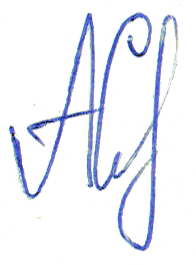
\includegraphics[width=10mm]{Подпись-Спиридонов.png}}%
\hspace*{8mm}%
{\large /}% 
\raisebox{-1mm}{\hbox to 0pt{\rule{40mm}{0.4pt}}}% 
~~А.А.\,Спиридонов%
\hspace*{3cm}%
\textbf{Дата} 
\raisebox{-1mm}{\hbox to 0pt{\rule{4cm}{0.4pt}}}% 
~~<<\,11\,>> июня 2020 г.

\bigskip

~~~~~~М.П.



 
\end{document}
